\documentclass{article}

\usepackage{amsmath, graphicx}

\title{Homework4 Report}
\author{Qi Liu}
\date{\today}

\begin{document}

\maketitle

\section{PAC Learning}
True, PAC says that the error can be less that $\epsilon$ for any $\epsilon>0$, but $\epsilon$ must be positive and can not reduce to zero.

\section{L2 Norm}

\subsection{Linear Regression}
Calculate the partial derivative of $J(\theta)$ respect to $\theta$, we get
$$\frac{\partial}{\partial\theta}J(\theta)= \frac{\partial}{\partial\theta}(y-X\theta)^T(y-X\theta)+ \lambda\frac{\partial}{\partial\theta}||\theta||^2_2= 2(X^TX\theta-X^Ty)+2\lambda\theta.$$ Set the partial derivative to 0, we get 
\begin{align*}
\frac{\partial}{\partial\theta}J(\theta)&=0 \\
2(X^TX\theta-X^Ty)+2\lambda\theta&=0 \\
X^TX\theta+\lambda\theta&=X^Ty \\
(X^TX+\lambda I)\theta&=X^Ty \\
\theta&=(X^TX+\lambda I)^{-1}X^Ty
\end{align*}

\subsection{Logistic Regression}
Calculate the partial derivative of $l(\theta)$ respect to $\theta$, we get
$$\frac{\partial}{\partial\theta}l(\theta)=\frac{\partial}{\partial\theta} \log\prod_{i=1}^mh_\theta(x^{(i)})^{y^{(i)}}(1-h_\theta(x^{(i)}))^{1-y^{(i)}}- \lambda\frac{\partial}{\partial\theta}||\theta||^2_2=\sum_{i=1}^m[y^{(i)}- h_\theta(x^{(i)})]x^{(i)}-2\lambda\theta.$$ Thus the updating rule for $\theta$ is $$\theta_{t+1}=\theta_{t}+\alpha(\sum_{i=1}^m[y^{(i)}- h_{\theta_t}(x^{(i)})]x^{(i)}-2\lambda\theta_t)$$ where $\alpha$ is the learning rate.

\section{GEM Algorithm}

\subsection{Correctness of GEM algorithm}
First, by Jensen's inequality, we can get $$\ell(\theta^{(t+1)})\ge\sum_i\sum_{z^{(i)}}Q_i(z^{(i)})\log \frac{p(x^{(i)},z^{(i)};\theta^{(t+1)})}{Q_i(z^{(i)})}.$$ And in the M-step of GEM algorithm, the $\alpha$ is chosen small enough that we do not decrease
the objective function, which means $\forall i$, $$p(x^{(i)},z^{(i)};\theta^{(t+1)}) \ge p(x^{(i)},z^{(i)};\theta^{(t)}).$$ This implies $$\sum_i\sum_{z^{(i)}}Q_i(z^{(i)})\log \frac{p(x^{(i)},z^{(i)};\theta^{(t+1)})}{Q_i(z^{(i)})} \ge \sum_i\sum_{z^{(i)}}Q_i(z^{(i)})\log \frac{p(x^{(i)},z^{(i)};\theta^{(t)})}{Q_i(z^{(i)})}.$$ And in the E-step, the $Q$ is chosen to satisfy $$\ell(\theta^{(t)})=\sum_i\sum_{z^{(i)}}Q_i(z^{(i)})\log \frac{p(x^{(i)},z^{(i)};\theta^{(t)})}{Q_i(z^{(i)})}.$$ Thus we have $\ell(\theta^{(t+1)})\ge\ell(\theta^{(t)})$.

\subsection{Gradient Ascent}
We think the problem statement has a little mistakes. There are no such $Q_i(z^{(i)})$ in the gradient ascent. We think the correct updating rule for the gradient ascent should be $$\theta:=\theta+\alpha\nabla_\theta\ell(\theta) =\theta+\alpha\nabla_\theta\sum_i\log\sum_{z^{(i)}}p(x^{(i)},z^{(i)};\theta).$$
Assume we use the same learning rate $\alpha$ for gradient ascent and GEM algorithm. The updating part in gradient ascent is
\begin{align*}
\nabla_\theta\sum_i\log\sum_{z^{(i)}}p(x^{(i)},z^{(i)};\theta)&=
\sum_i\frac{1}{\sum_{z^{(i)}}p(x^{(i)},z^{(i)};\theta)} \sum_{z^{(i)}}\nabla_\theta p(x^{(i)},z^{(i)};\theta) \\
&=\sum_i\frac{1}{p(x^{(i)};\theta)}\sum_{z^{(i)}}\nabla_\theta p(x^{(i)},z^{(i)};\theta).
\end{align*}
The updating part for GEM algorithm is $$\nabla_\theta\sum_i\sum_{z^{(i)}}Q_i(z^{(i)})\log \frac{p(x^{(i)},z^{(i)};\theta)}{Q_i(z^{(i)})}=
\sum_i\sum_{z^{(i)}}\frac{Q_i(z^{(i)})}{p(x^{(i)},z^{(i)};\theta)} \nabla_\theta p(x^{(i)},z^{(i)};\theta).$$ We know in the E-step of GEM algorithm, the $Q$ will be chosen to satisfy $$Q_i(z^{(i)})=p(z_{(i)}|x_{(i)};\theta)= \frac{p(z_{(i)},x_{(i)};\theta)}{p(x_{(i)};\theta)},$$ then
\begin{align*}
\sum_i\sum_{z^{(i)}}\frac{Q_i(z^{(i)})}{p(x^{(i)},z^{(i)};\theta)} \nabla_\theta p(x^{(i)},z^{(i)};\theta)&=
\sum_i\sum_{z^{(i)}}\frac{1}{p(x^{(i)};\theta)} \nabla_\theta p(x^{(i)},z^{(i)};\theta) \\
&=\sum_i\frac{1}{p(x^{(i)};\theta)}\sum_{z^{(i)}}\nabla_\theta p(x^{(i)},z^{(i)};\theta).
\end{align*}
Which means gradient ascent and GEM algorithm will update the same value.

\section{Clustering}
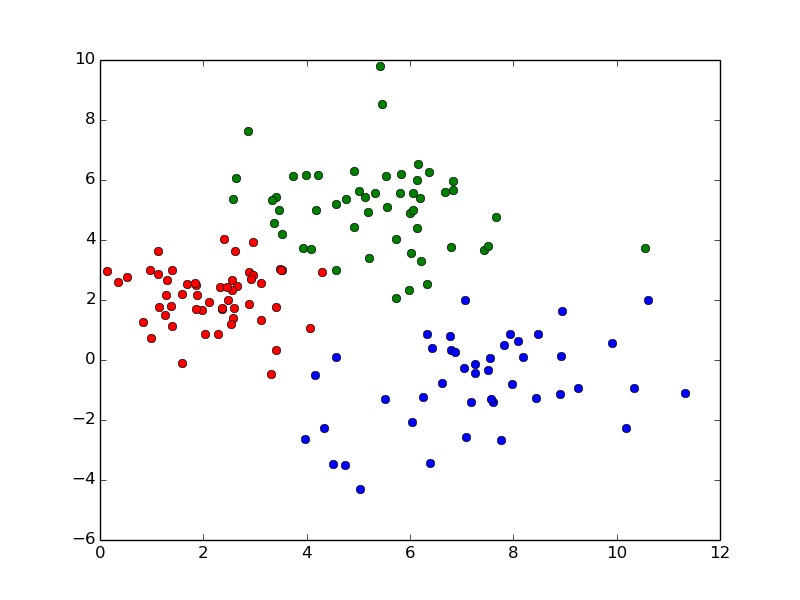
\includegraphics[width=0.5\textwidth]{../result/kmeans.jpg}
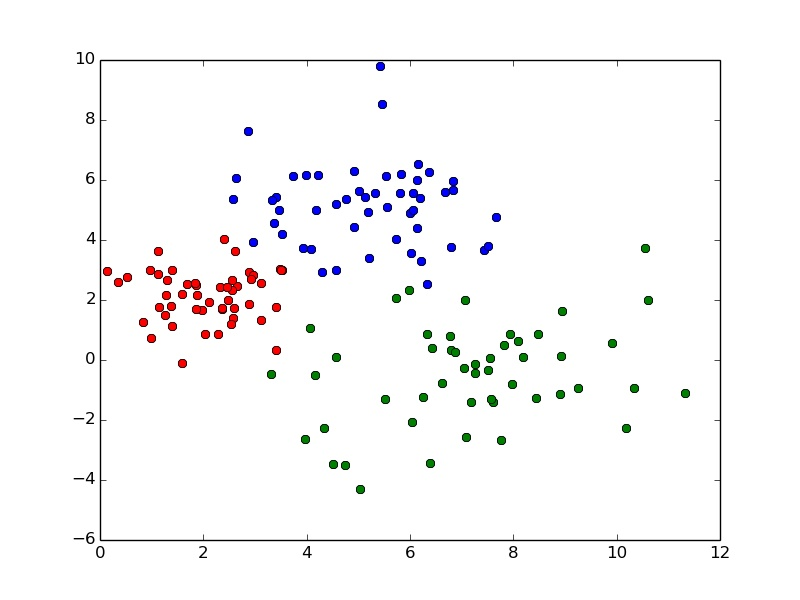
\includegraphics[width=0.5\textwidth]{../result/gmm.jpg}

The left figure is the clustering result of by using K-means and the right one is the result of GMM. The table below shows the parameters of two models.

\begin{center}
\begin{tabular}{|c|c|c|c|c|c|c|c|}
\hline \bf{Cluster} & \multicolumn{2}{c|}{\bf{K-means}} & \multicolumn{5}{c|}{\bfseries{GMM}} \\
\hline
number & \multicolumn{2}{c|}{center} & weight & \multicolumn{2}{c|}{mean} & \multicolumn{2}{c|}{covariance} \\
\hline 1 & 2.188 & 2.135 & 0.327 & 2.079 & 2.167 & 0.795 & 0.731 \\
\hline 2 & 5.343 & 5.077 & 0.331 & 7.121 & -0.410 & 3.767 & 3.048 \\
\hline 3 & 7.306 & -0.732 & 0.341 & 5.102 & 5.099 & 1.794 & 2.037 \\
\hline
\end{tabular}
\end{center}

We can see K-means and GMM all get good result, they only differ on some boundary points.

\end{document}